The goal of this section is to give the necessary information to understand the rest of the thesis. Debugging is a complicated process that is made much harder by distributing the system to more than one physical location.

\section{Flink Framework}
\label{flinkFramework}

Flink is a Framework for processing applications that are distributed across multiple computers. This part will lay out the foundations of the Flink Framework.
Flink applications have a simple base structure that is used by the developer. Each application defines tasks which have a particular structure. Each task has an input and output stream. These are called source and sink. Because both the source and sink of these tasks are streams, they can be attached to each other thus creating a data flow from task to task until the wanted end state is reached.

\begin{figure}[h!]
    \centering
      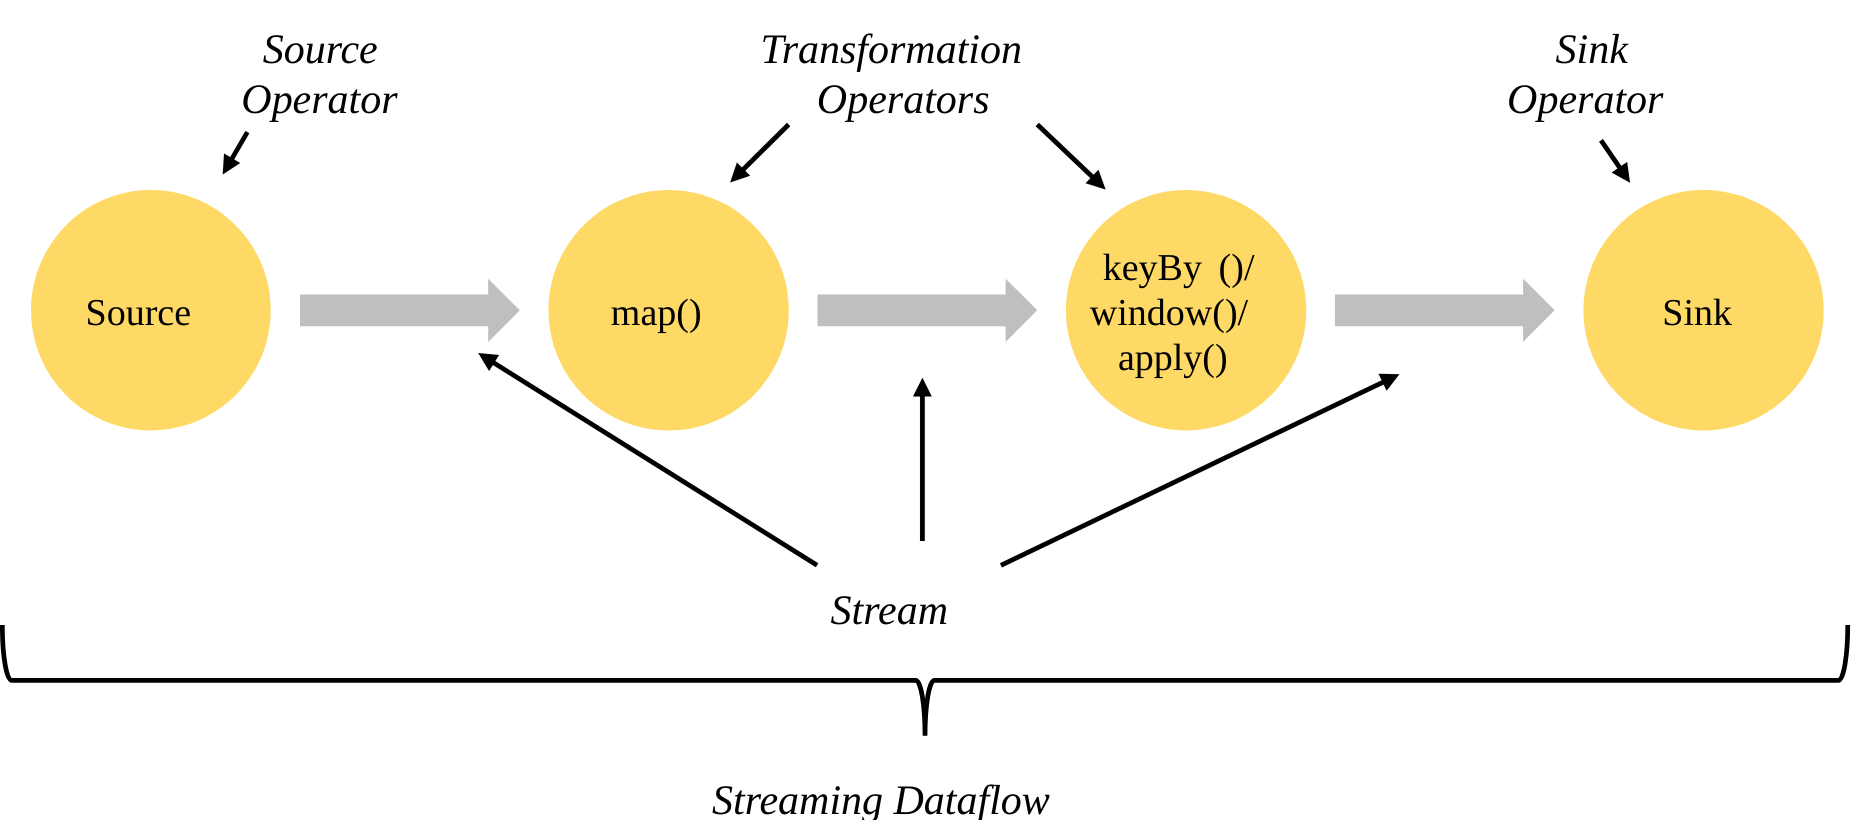
\includegraphics[width=0.9\textwidth]{rw_simpleDataflowInFlink.png}
      \caption{Simple Dataflow in Flink}
      \label{simpleDataflowInFlink}
\end{figure}

Figure \ref{simpleDataflowInFlink} shows a basic program flow. On the left side, it starts with a source. The source is then transferred over a data stream to the first task. The map operation is executed, and the result is sent over a data stream to the next task where the same procedure will start again. The resulting data in this example is the sink, meaning we reached the end of the program. The sink will typically be connected to a database or some other kind of Technology for preserving the data. The most basic option would be to write the sink onto the standard output on the console.

Until now the system can only be distributed by having the different tasks on different physical computers. This distribution process will not suffice when the amount of input data gets too high. To achieve real distribution in the application, each task can be run multiple times as so called subtasks. These subtasks run as a single thread in the JVM and are managed by a task manager. Task Managers connect to a Job Manager which coordinates the distributed execution. The data flow from one subtask to another can either be one to one or as a redistributing data flow. A redistributing data flow is necessary to achieve an even distribution of data at the next subtasks.

\begin{figure}[h!]
    \centering
      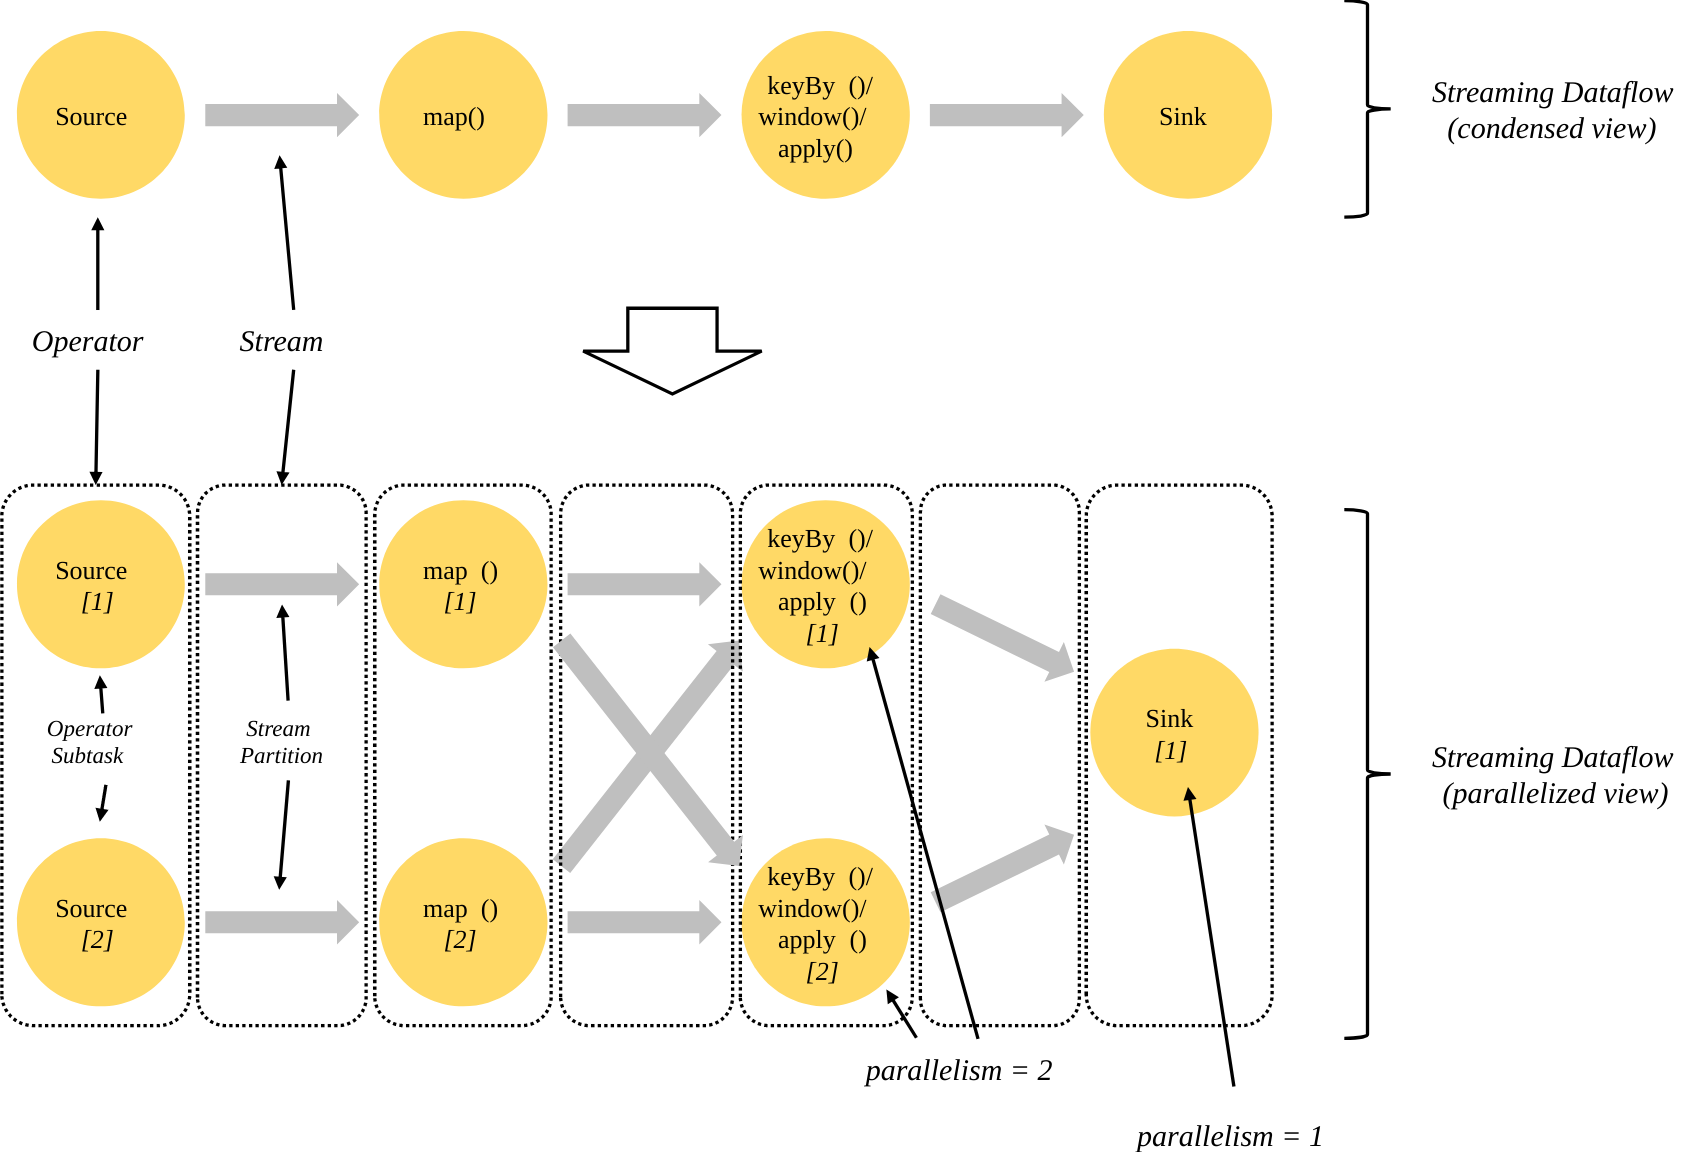
\includegraphics[width=0.9\textwidth]{rw_distributedDataflowInFlink.png}
      \caption{Distributed Dataflow in Flink}
      \label{distributedDataflowInFlink}
\end{figure}

Figure \ref{distributedDataflowInFlink} presents the same example as figure \ref{simpleDataflowInFlink} just with the subtasks shown as well. The map task is a vital step in each application as it connects the data from each subtask with each other. It is easily understood be a simple example. In an application that counts how often each word is in a text, it would only split the text at each space symbol. The redistributing data flow would then create an even distribution in the next node which specifies what to count by (id task) and applies a particular aggregation function to the "apply" operation. The result is then sent to the sink operator. This explanation is a simplification of the actual MapReduce model. For a complete overview see \cite{todo}.

\subsection{Stream vs. Batch}

Apache Flink is primarily a stream processing framework, although you can also use batch processing. As it makes a big difference in the infrastructure of the framework, it is important to lay out the differences between the two.

\paragraph{Stream Processing} uses as the names suggest a stream to acquire the data. A stream is an endless sequence of data that can be utilised both as an input and output. As there is no end, it makes it tough to use algorithms on it. Flink uses "Windows" to solve this problem. These windows offer a frame for the operations to only use data that was received in each window. Windows can be programmed and provide various ways to define the frame. The simplest way would be just to give a timeframe, but one could also build complex structures.

\paragraph{Batch Processing} on the other hand has set boundaries, and it is evident how much data is sent and where it ends. To support batch processing as well in the Flink Framework the windows can be programmed to have the same size as the data you want to batch processed. That way even though Flink uses streams it still supports batch processing.
